\subsection{Feinkonzept}
\label{sec:Feinkonzept}

Durch die iterative Erarbeitung des Feinkonzeptes und der Genehmigung des
Projektes durch die Fakultätsleitungsrunde, wurde der Abschluss des Feinkonzepts
erfolgreich erreicht. Das endgültige Feinkonzept stellt sich folgendermaßen dar:

Die Realisierung des Projektes erfolgt mit der Umsetzungsmöglichkeit des
virtuellen Rundgangs durch den Campus im Stile von Google Street View. Dabei ist
es möglich sich virtuell durch den Campus zu bewegen. Dieses Projekt soll am
14.07.2014 abgeschlossen werden. Im Bezug auf Datenschutz werden die
Datenschutzrichtlinien beachtet, welche im Anhang ~\ref{sec:Datenschutzrichtlinien} einsehbar sind. Die
Nachhaltigkeit dieses Projektes wird gewährleistet, indem die Möglichkeit
besteht, dass andere Personen die Anwendung administrieren können. Dies wird über
einen Administrationsbereich realisiert, der die notwendigen Funktionen zur
Anwendungspflege bereitstellt.\footnote{siehe \citet{lastenheft2013}} Hierzu
wird ebenfalls eine Dokumentation über die Nutzung der Anwendung und der
Administration angefertigt und bei Projektabschluss übergeben.

Ein Ausblick auf die zu enstehende Anwendung zeigt eine bestehende 
Google Street View Anwendung:

\clearpage
\begin{figure}[htb] 
\centering
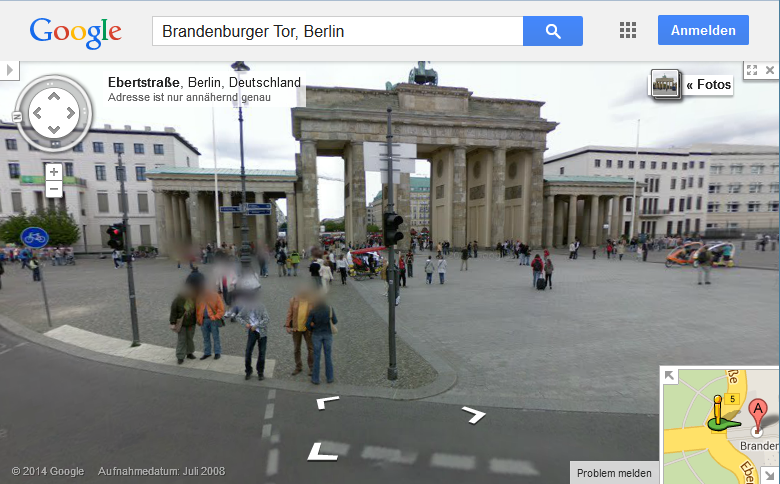
\includegraphics[width=0.7\textwidth]{GoogleStreetView.png}
\caption[Google Street View]{Google Street View\protect\footnotemark}
\label{fig:GoogleStreetView}
\end{figure}
\footnotetext{Bildschirmfoto von \url{https://maps.google.de/}}

Durch das erarbeitete Feinkonzept sind die Details des Projektes an dieser Stelle bekannt.
Auf diesen Details aufbauend wird ein Zielkatalog erstellt, der die erarbeiteten Projektziele
mit Zielindikatoren verknüpft.